\documentclass[dvipdfmx,autodetect-engine, 12pt]{jsarticle}

\usepackage{ulem} % 取消線を引くためのパッケージ
\usepackage[dvipdfmx]{graphicx} % 画像を挿入するためのパッケージ
\usepackage{array} % 表の幅指定や自動改行に必要
\usepackage{enumitem}
\usepackage{amsmath}

% --- 考文献用の設定 ---
\usepackage[backend=biber, style=numeric]{biblatex} % biblatexパッケージの使用
\addbibresource{source.bib} % 先ほど作った別ファイルを指定（拡張子まで書く）
\usepackage{url} % WebサイトのURLを綺麗に出力するため

% --- section の文字サイズを小さくする設定 ---
\makeatletter
\renewcommand{\section}{%
  \@startsection{section}{1}{\z@}%
  {1.5ex \@plus .5ex \@minus .2ex}% 前の行との隙間
  {0.5ex \@plus .3ex}% 下の行との隙間
  {\normalfont\normalsize}% ← ここでサイズを \Large（少し大きめ）に指定
}
\makeatother

\begin{document}

% 課題のタイトル
\begin{center}

    {\LARGE \bfseries 課題③\,ARPおよびICMPパケットの解析\par}

\end{center}

\vspace{1cm}

{\LARGE \uline{目的}} 

\vspace{1cm}

{\LARGE \uline{事前準備}} 

\begin{enumerate}
    \item server と router の VM を起動する．
    \item arp と ping コマンドで利用されるプロトコルを調査する.
\end{enumerate}

\vspace{1cm}

{\LARGE \uline{手順}} 

\begin{enumerate}
    \item arpとpingコマンドで, どのプロトコルが利用されるのか調査し, 
          特に通信の開始から終了までに, 通信元と通信先との間に, OSI参照モデルのどの層で, 
          どのような手順で, どのように, どのような情報が, やり取りされるのか詳細を調べ, 整理しなさい.

        \vspace{\baselineskip}

        \quad arpコマンドは, ARP(Address Resolution Protocol)によって, ARPテーブルに記録された情報を表示・編集するためのコマンドである\cite{bashdo_arp}.
        ARPとは, ネットワークがコンピュータのIPアドレスと物理的なマシンアドレスを変換（解決）するために使用される一般的な手法であり\cite{kinsta_arp}, 
        宛先ホストのIPアドレスを手がかりに, 次に送るべき機器のMACアドレスを調べる.
        送信元IPアドレスと宛先IPアドレスを比較して, 宛先IPアドレスが同じネットワーク上にあるときには, その宛先IPアドレスのMACアドレスを調べ, 
        宛先IPアドレスが異なるネットワーク上にある場合には, 次に送るルータのIPアドレスからMACアドレスを調べる.
        ARPパケットのフォーマットと各フィールドの説明をそれぞれ図\ref{fig:arp_packet_format}と表\ref{tab:arp_fields}に示す.
        \\
        

        \begin{figure}[htbp]
            \centering
            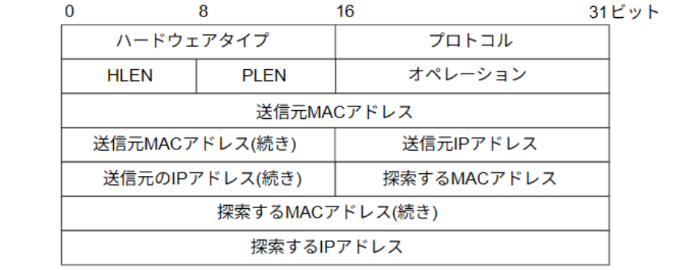
\includegraphics[width=0.8\textwidth]{imgs/arp_packet_format.png} 
            \caption{ARPによるアドレス解決の仕組み（\cite{nw_text_r08}より引用・改変）}
            \label{fig:arp_packet_format}
        \end{figure}

        \begin{table}[htbp]
            \centering
            \caption{ARPパケットのフィールド構成（\cite{nw_text_r08}を参照に作成）}
            \label{tab:arp_fields}
            % p{8cm} を m{8.5cm} に変更し、垂直方向の中央揃えと幅の調整を行います
            \begin{tabular}{|c|c|m{8.5cm}|}
                \hline
                \multicolumn{1}{|c|}{フィールド名} & ビット数 & \multicolumn{1}{c|}{内容} \\ \hline
                ハードウェアタイプ & 16 & どのようなデータリンクを使用しているかを示す． \\ \hline
                プロトコルタイプ   & 16 & ネットワーク層のプロトコルについて示す． \\ \hline
                HLEN              & 8  & ハードウェアアドレスの長さを示す． \\ \hline
                PLEN              & 8  & プロトコルアドレスの長さを示す． \\ \hline
                オペレーション     & 16 & ARP要求パケットかARP応答パケットかを示す．\newline ARP要求パケットの場合は1，\newline ARP応答パケットの場合は2． \\ \hline
                \begin{tabular}{@{}c@{}}送信元MAC\\アドレス\end{tabular}  & 48 & 送信元MACアドレスを示す．\newline ARP応答パケットでは，ここにARP要求パケットで求めていたMACアドレスが設定されて返される． \\ \hline
                \begin{tabular}{@{}c@{}}送信元IP\\アドレス\end{tabular}   & 32 & 送信元IPアドレス． \\ \hline
                \begin{tabular}{@{}c@{}}探索するMAC\\アドレス\end{tabular} & 48 & 探索するMACアドレスを示す．ARPパケットではここが分からないので，通常は0の値が設定されている． \\ \hline
                \begin{tabular}{@{}c@{}}探索するIP\\アドレス\end{tabular}  & 32 & ARP要求パケットでは，探索するIPアドレスを示し，ARP応答パケットでは，宛先（要求パケットの送信元）のアドレスが設定される． \\ \hline
            \end{tabular}
        \end{table}

        \quad 続いて, ARPによってアドレス解決を行う際の手順について示す.
        ここではホストAがホストBのMACアドレスを解決しようとしているものとする.

        \vspace{\baselineskip}

        \begin{enumerate}[label=\textcircled{\scriptsize\arabic*}]
            \item ホストAは探索するIPアドレスにホストBのIPアドレスを指定したARP要求パケットをネットワークにブロードキャストする.
            \item ホスト B は ARP 要求パケットを受け取ると, ホスト A に対して自身の NIC に割り当てられている MAC アドレスを ARP ユニキャストする.
            \item ホスト A は ARP 応答パケットを受け取り, そこに記述される MAC アドレスはコンピュータ内の ARP テーブルに登録され, 数分間キャッシュされる. 一度登録されるとキャッシュされている間は ARP の再問い合わせが実行されることはない.
        \end{enumerate}
    
    \item 両 VM で console を開く．

    \item 次のコマンドを実行して，IP アドレスを確認する．\\
          \texttt{\# ifconfig -a}\\
          {\small ※ Request timed out.が表示され所定の情報が得られない場合は，各 PC のフィルタリングの設定を確認する．}
    
    \quad
    図\ref{fig:router_ifconfig}, \ref{fig:server_ifconfig}にそれぞれ router と server の ifconfig コマンドの実行結果を示す. 
    また, この結果から読み取れる情報についてまとめたものを表\ref{tab:ifconfig_info}に示す.
    routerは10.6.158.0/24のネットワークに属するインターフェースeth1と
    192.168.100.0/24のネットワークに属するインターフェースeth0を持っており,
    serverは192.168.100.0/24のネットワークに属するインターフェースeth0を持っていることが読み取れる.

    \begin{figure}[htbp]
        \centering
        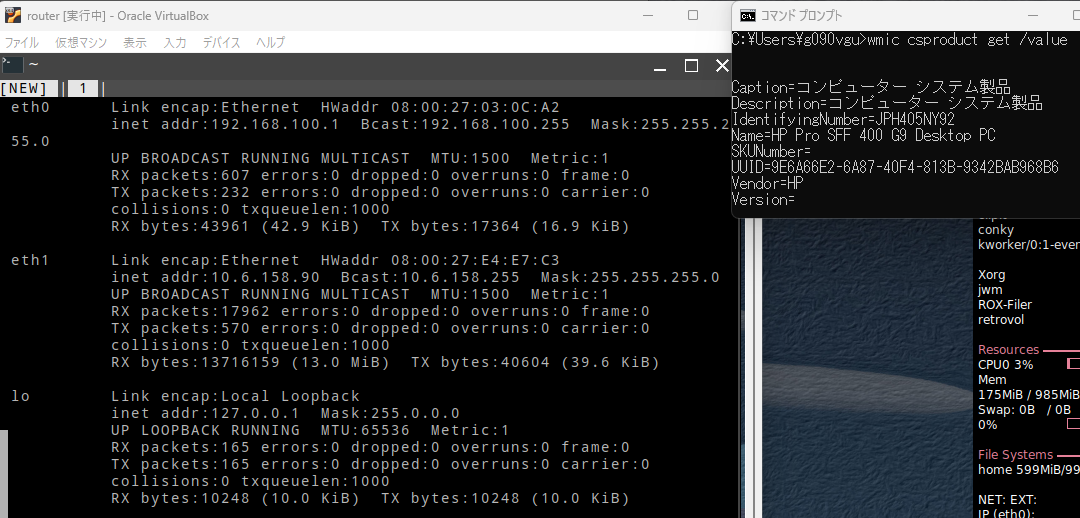
\includegraphics[width=0.8\textwidth]{imgs/router_ifconfig.png} 
        \caption{router の ifconfig コマンドの実行結果}
        \label{fig:router_ifconfig}
    \end{figure}

    \begin{figure}[htbp]
        \centering
        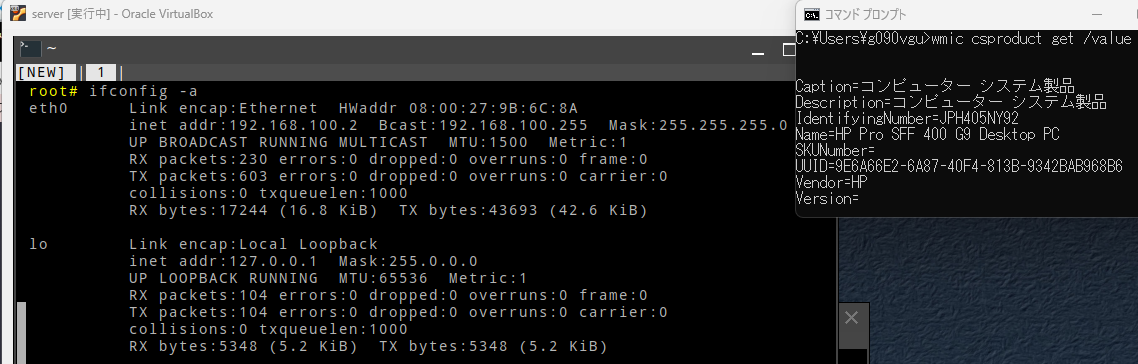
\includegraphics[width=0.8\textwidth]{imgs/server_ifconfig.png} 
        \caption{server の ifconfig コマンドの実行結果}
        \label{fig:server_ifconfig}
    \end{figure}

    \begin{table}[htbp]
        \centering
        \caption{ifconfig コマンドの実行結果から読み取れる情報のまとめ}
        \label{tab:ifconfig_info}
        \begin{tabular}{|c|c|c|c|}
            \hline
            VM & インターフェース名 & IPアドレス & MACアドレス \\ \hline
            router & eth1 & 10.6.158.90 & 08:00:27:03:0c:a2 \\ \hline
            router & eth0 & 192.168.100.1 & 08:00:27:e4:e7:c3 \\ \hline
            server & eth0 & 192.168.100.2 & 08:00:27:9b:6c:8a \\ \hline
        \end{tabular}
    \end{table}    
    
    \item マシン間で ping を実行する．\\
          \texttt{\# ping 別の VM の IP アドレス}

    \quad
    VM間でのpingの実行結果を図\ref{fig:ping_router2server_before}, \ref{fig:ping_server2router_before}に示す.
    いずれの場合においても, 全パケットに対して応答が帰ってきていることが0\%\, packet\, lossという出力から読み取れる.
    
    \begin{figure}[htbp]
        \centering
        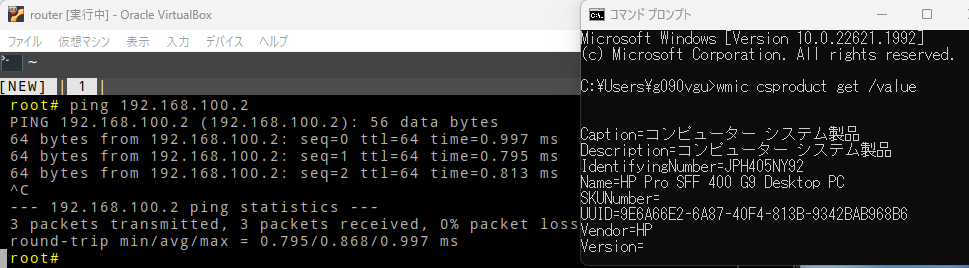
\includegraphics[width=0.8\textwidth]{imgs/router2server_ping.png} 
        \caption{router から server への ping の実行結果}
        \label{fig:ping_router2server_before}
    \end{figure}

    \begin{figure}[htbp]
        \centering
        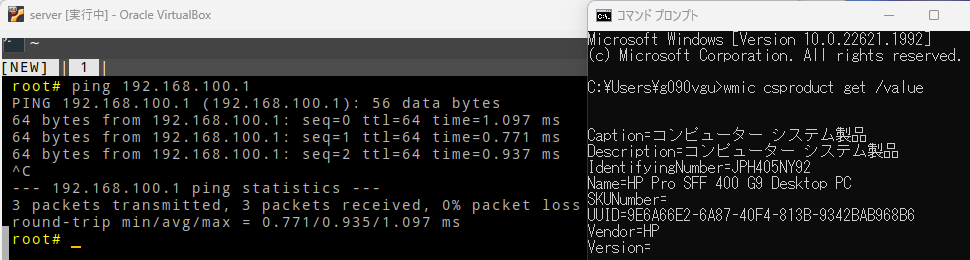
\includegraphics[width=0.8\textwidth]{imgs/server2router_ping.png} 
        \caption{server から router への ping の実行結果}
        \label{fig:ping_server2router_before}
    \end{figure}
        
    \item 両方の VM で次のコマンドを実行し，ARP キャッシュの内容を確認する．\label{item:arp_cache_check1}\\
          \texttt{\# arp -an}
    \item 確認後，次のコマンドを実行し，server の arp キャッシュの内容をクリアする．\label{item:arp_cache_clear}\\
          \texttt{\# arp -d IP アドレス（ARP キャッシュに残っている IP アドレス）}
    \item 再度，ARP キャッシュの内容を確認し，クリアされていることを確認する．\label{item:arp_cache_check2}\\
          {\small ※ 組織外側のネットワークの端末に関するキャッシュは消せなくてもよい．}

    図\ref{fig:router_arp}, \ref{fig:server_arp}にそれぞれ router と server の 
    手順\ref{item:arp_cache_check1}, \ref{item:arp_cache_clear}, \ref{item:arp_cache_check2}
    の実行結果を示す.
    それぞれキャッシュがクリアされた後では, 192.168.100.0/24に属するarpテーブルの内容が空になっていることがわかる.

    \begin{figure}[htbp]
        \centering
        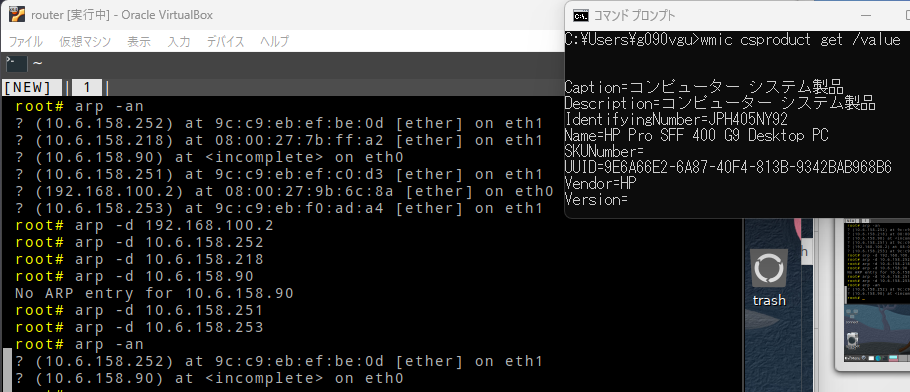
\includegraphics[width=0.8\textwidth]{imgs/router_arp.png} 
        \caption{router の ARP キャッシュ}
        \label{fig:router_arp}
    \end{figure}

    \begin{figure}[htbp]
        \centering
        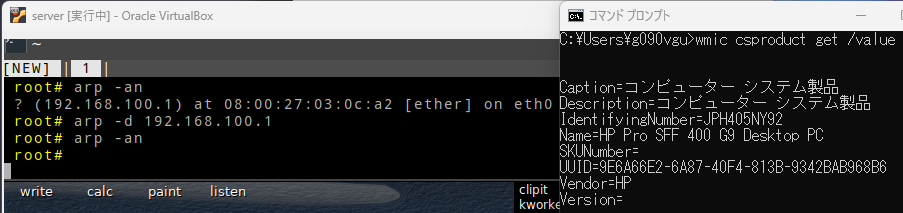
\includegraphics[width=0.8\textwidth]{imgs/server_arp.png} 
        \caption{server の ARP キャッシュ}
        \label{fig:server_arp}
    \end{figure}
    
    \item server の VM で Wireshark-gtk を起動する．\label{item:wireshark_on}
    \item \text{[Wireshark]}のメニューの\text{[Capture]}→\text{[Start]}を実行し，キャプチャを開始する.\label{item:wireshark_start}\\
          {\small ※ Capture Interfaces で router と接続しているインターフェース(デバイス)を指定すること}
    \item server から router へ ping を実行する．\label{item:ping_server2router}
    
    図\ref{fig:ping_server2router_for_packet_analyze}, \ref{fig:ping_wireshark}
    にserverからrouterへのpingの実行結果とそれによって生じたパケットの一覧を示す.

    \begin{figure}[htbp]
        \centering
        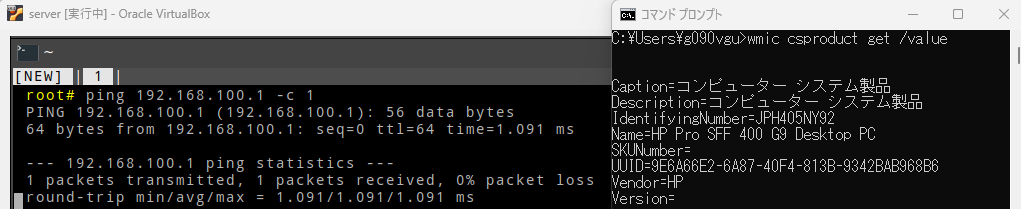
\includegraphics[width=0.8\textwidth]{imgs/server_ping_for_packet_analyze.png} 
        \caption{Wiresharkでキャプチャされたpingによって生じた通信の一覧}
        \label{fig:ping_server2router_for_packet_analyze}
    \end{figure}

    \begin{figure}[htbp]
        \centering
        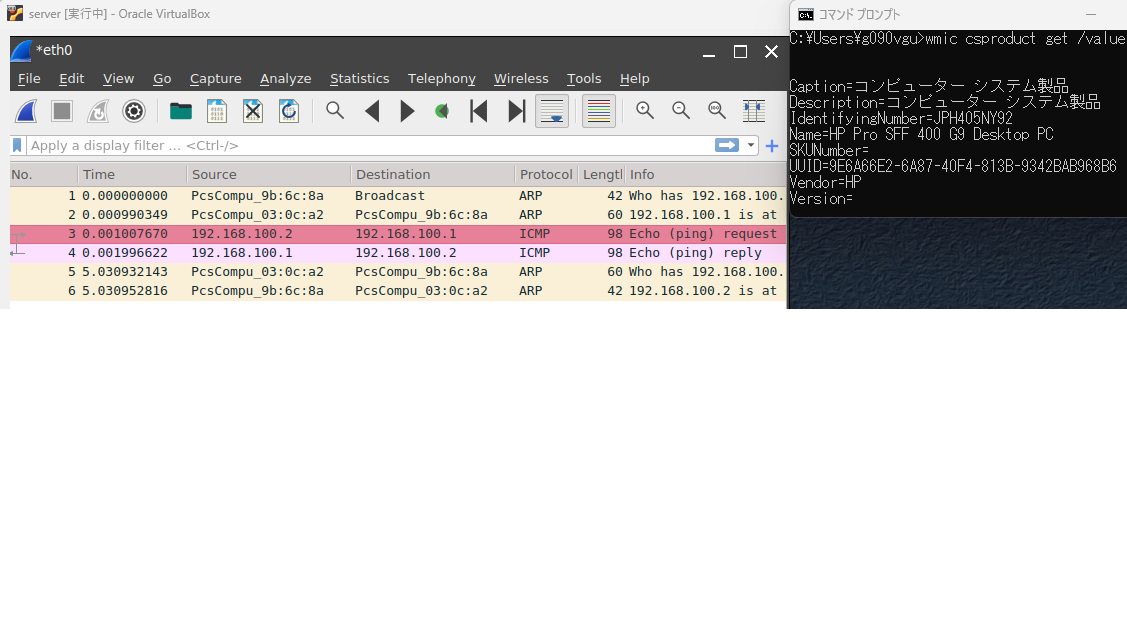
\includegraphics[width=0.8\textwidth]{imgs/ping_wireshark.png} 
        \caption{Wiresharkでキャプチャされたpingによって生じた通信の一覧}
        \label{fig:ping_wireshark}
    \end{figure}

    図\ref{fig:ping_server2router_for_packet_analyze}から, ここでもパケットは損失することなく, 正常に通信できたことがわかる.
    図\ref{fig:ping_wireshark}から, pingによって生じた通信では, ARPのパケットが送受信された後に, ICMPのパケットが送受信されていることがわかる.

    \item \text{[Capture]}→\text{[Stop]}を実行してキャプチャを停止し，ARPによって生じた通信を確認し，調査結果より想定される手続きで情報が端末間でやり取りされているか解析しなさい．
    
    \quad
    図\ref{fig:arp_request_packet}, \ref{fig:arp_reply_packet}にARPによって生じた通信のパケットであるARPリクエストパケットとARPリプライパケットを示す.

    \begin{figure}[htbp]
        \centering
        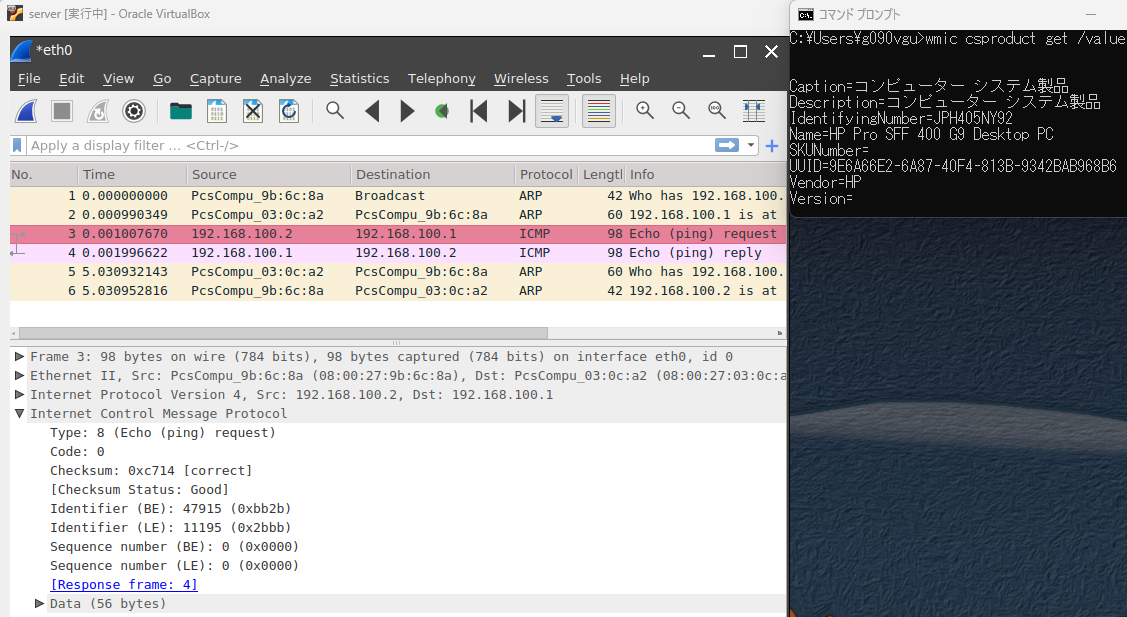
\includegraphics[width=0.8\textwidth]{imgs/server_ping_request_packet.png} 
        \caption{ARPリクエストパケット}
        \label{fig:arp_request_packet}
    \end{figure}

    \begin{figure}[htbp]
        \centering
        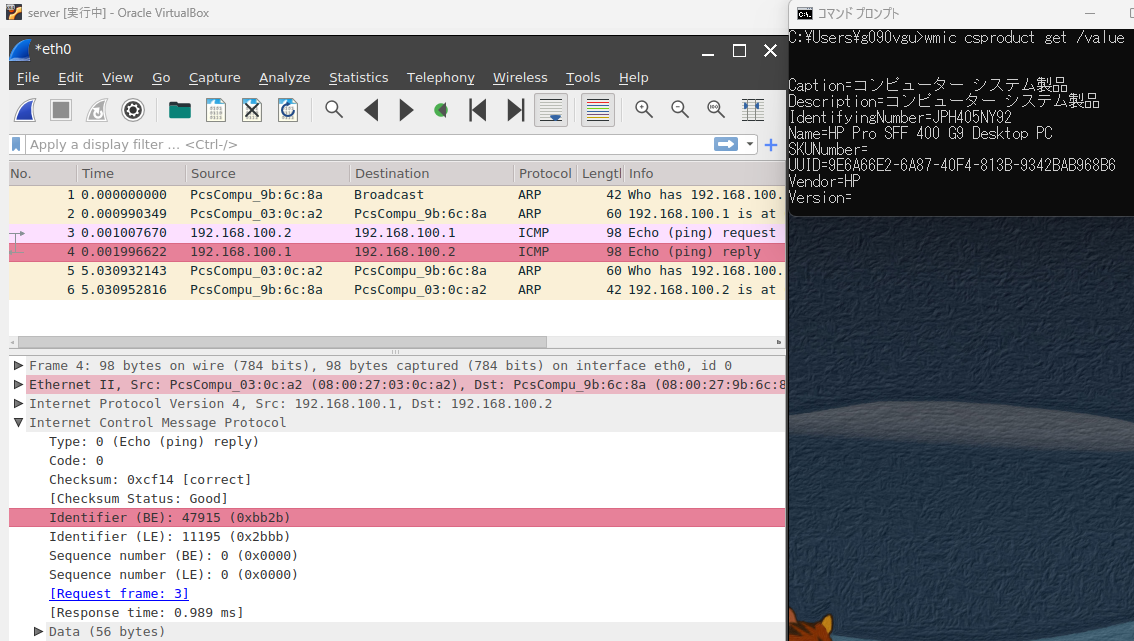
\includegraphics[width=0.8\textwidth]{imgs/server_ping_reply_packet.png} 
        \caption{ARPリプライパケット}
        \label{fig:arp_reply_packet}
    \end{figure}

    まず, パケットのフォーマットについて比較を行う. 
    図\ref{fig:arp_packet_format}に示したARPパケットのフォーマットは図\ref{fig:arp_request_packet}, \ref{fig:arp_reply_packet}から確認できる実際に得られたパケットのフォーマットと完全に一致していることが確認できる.
    オペレーション(opcode)について確認すると, それぞれ1,2の値が設定されており, それぞれARP要求パケットとARP応答パケットであることがわかる.
    図\ref{fig:arp_request_packet}においては, 探索するIPアドレス(Target IP address)のフィールドにrouterのIPアドレスである192.168.100.1,
    



    

    \item 次に，ping コマンドによって生じた通信の内容を確認し，調査結果より想定される手続きで情報がやり取りされているか端末間で解析しなさい．

    

    \item 再度，ARP キャッシュの内容を確認する．
    \item 実験で得た結果（コマンド実行結果，キャプチャした結果など）を用いて，arp と ping を用いた通信の仕組み・手続きをレポートで報告しなさい．
\end{enumerate}

\newpage

% --- 参考文献リストの出力 ---
\printbibliography[title=参考文献]

\end{document}